\section{Experiment}
\subsection{Dataset and Settings}


% 本研究基于Deform-3D构建了600组锻造仿真数据集，重点控制初始温度场与锻造速度。通过模拟冷却过程获得10组非均匀初始温度场；通过参数$\theta=\{v_0,v_1,t_0,t_1\}$生成60组速度曲线$v_y(t)$。每个案例输出温度、应力、变形、损伤等多物理场数据，以点云形式存储，每时间步约5000个点，记录坐标$(x, y, z)$及各物理量。

This study established a dataset of 600 forging simulations using
Deform-3D, with controlled variations in the initial temperature field
and forging speed. Ten non-uniform initial temperature fields were
generated by simulating the cooling process. Sixty distinct speed
profiles $v_y(t)$ were produced by varying the parameters
$\theta = \{v_0, v_1, t_0, t_1\}$. Each simulation outputs multi-physics
field data (temperature, stress, strain, damage), stored as point clouds
containing approximately 5,000 points per time step. Each point records
its coordinates $(x, y, z)$ and the corresponding physical quantities.

\subsection{Evaluation of the Simulator}
% 为评估模型对物理场的预测精度，以应力场为例，将模型预测点云与有限元仿真结果对比。如图\ref{fig:model_result}所示，不同工况下预测与真实应力分布高度一致，表明模型能准确捕捉场量的空间分布特征。误差分析显示，偏差集中于局部区域且幅度较小。训练与测试阶段的均方误差分别为0.1780和0.2200，表明模型在场量预测中具有较好精度，能有效学习不同工况下的物理场分布规律。

The predictive accuracy of the surrogate model is evaluated by comparing
its stress field predictions against finite element simulation results.
As shown in Fig. \ref{fig:model_result}, the predicted and actual stress
distributions exhibit strong agreement under various working conditions,
demonstrating the model's capability to accurately capture spatial field
characteristics. Error analysis indicates that deviations are localized
and minimal. With mean squared errors of 0.1780 (training) and 0.2200
(testing), the model demonstrates high precision in field prediction and
effectively learns the distribution patterns of physical fields across
different conditions.

\begin{figure}[htbp]
\centerline{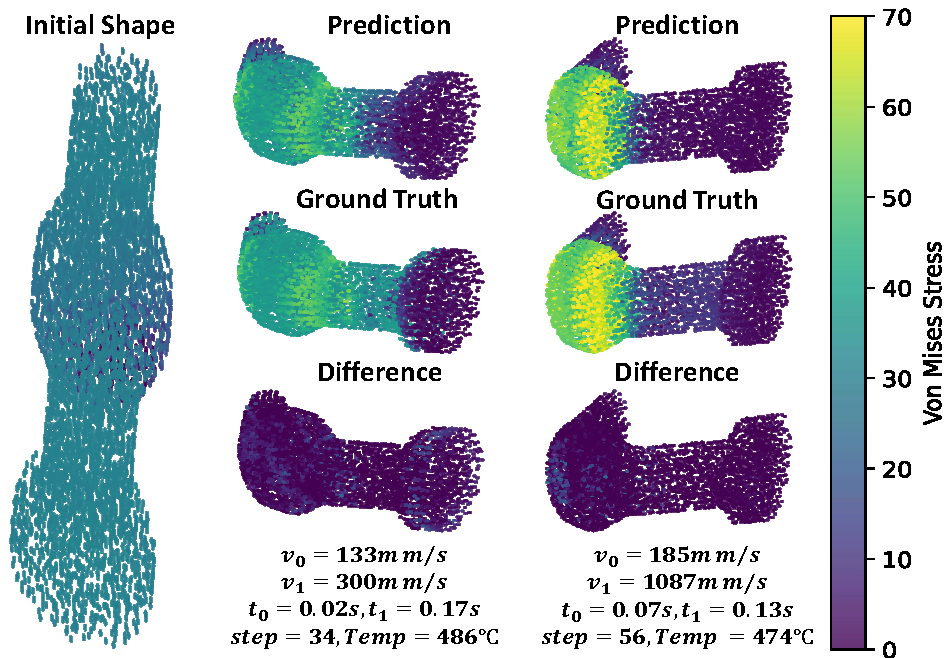
\includegraphics[width=\linewidth]{model_result-1.pdf}}
\caption{Comparison of model predictions and FEA results.}
\label{fig:model_result}
\end{figure}




\subsection{Evaluation on Offline RL}
% 强化学习结果如图\ref{fig:reward_a}与\ref{fig:damage_b}所示。平均奖励从波动上升至稳定正值（图\ref{fig:reward_a}），表明策略收敛；损伤值后期稳定低于$c_0=0.43$（图\ref{fig:damage_b}），满足安全约束。结果表明，该方法兼具优化能力与约束满足性，适用于锻造工艺决策。

The reinforcement learning results are shown in Figs. \ref{fig:reward_a}
and \ref{fig:damage_b}. The average reward rises from fluctuations to a
stable positive value (Fig. \ref{fig:reward_a}), indicating policy
convergence, while the damage value stabilizes below the threshold
$c_0 = 0.43$ (Fig. \ref{fig:damage_b}), confirming constraint
satisfaction. These results demonstrate that the proposed method
effectively balances optimization performance with safety compliance,
validating its applicability to forging process decision-making.



% \begin{figure}[htbp]
% \centerline{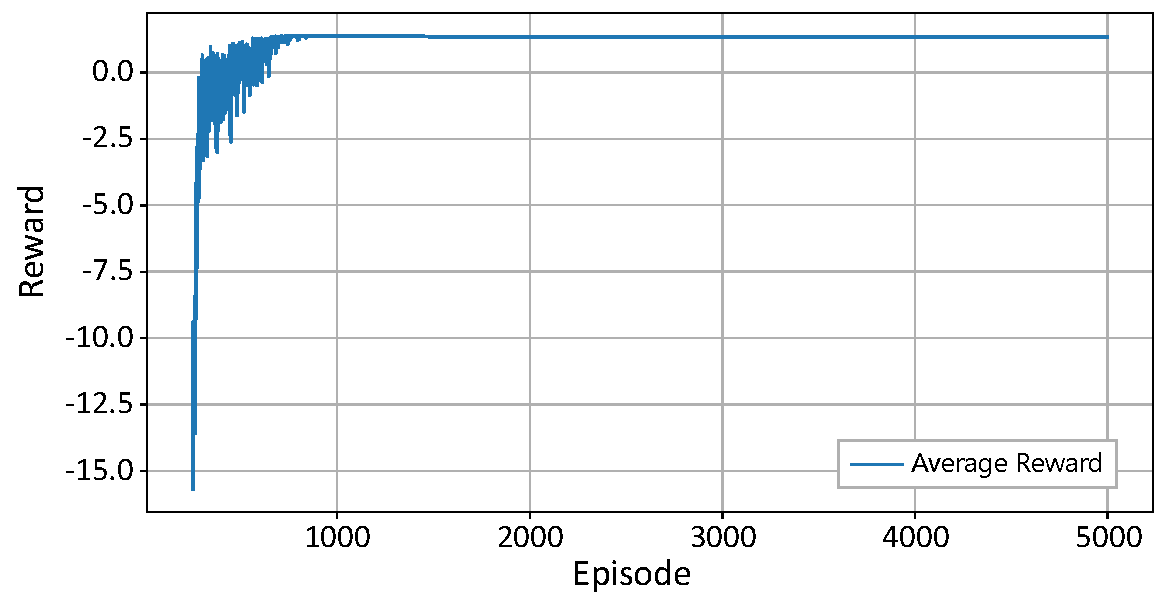
\includegraphics[width=\linewidth]{reward-1.pdf}}
% \caption{Training reward over epochs.}
% \label{fig:reward_a}
% \end{figure}


% \begin{figure}[htbp]
% \centerline{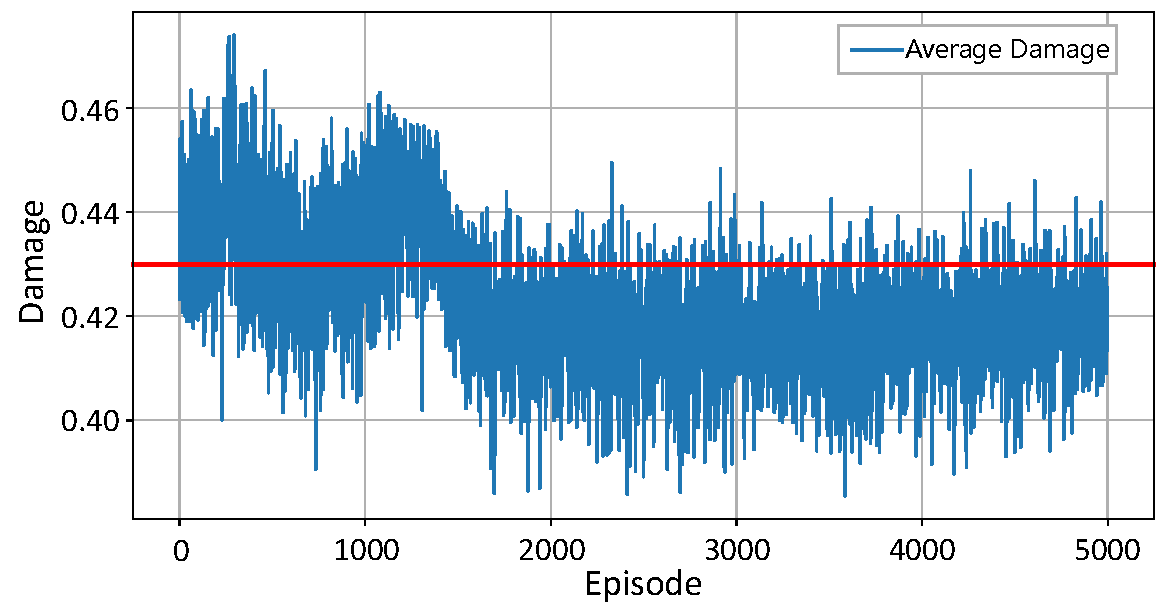
\includegraphics[width=\linewidth]{damage-1.pdf}}
% \caption{Training damage over epochs.}
% \label{fig:damage_b}
% \end{figure}

\begin{figure}[htbp]
    \centering
    \begin{subfigure}{0.48\columnwidth}
        \centering
        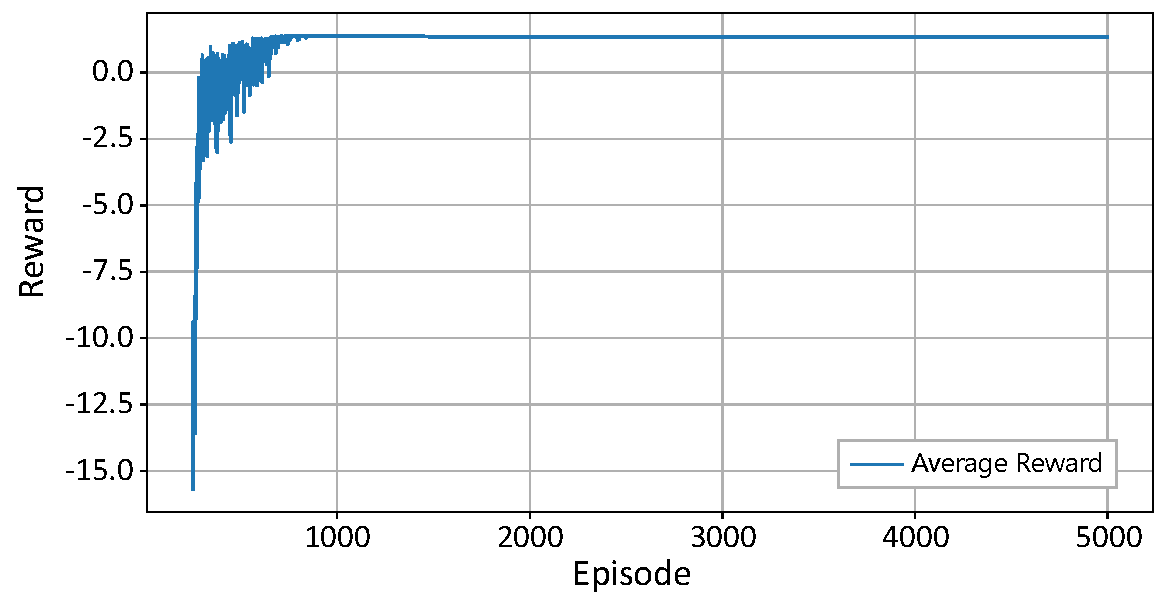
\includegraphics[width=\linewidth]{reward-1.pdf}
        \caption{Reward}
        \label{fig:reward_a}
    \end{subfigure}
    \hfill
    \begin{subfigure}{0.48\columnwidth}
        \centering
        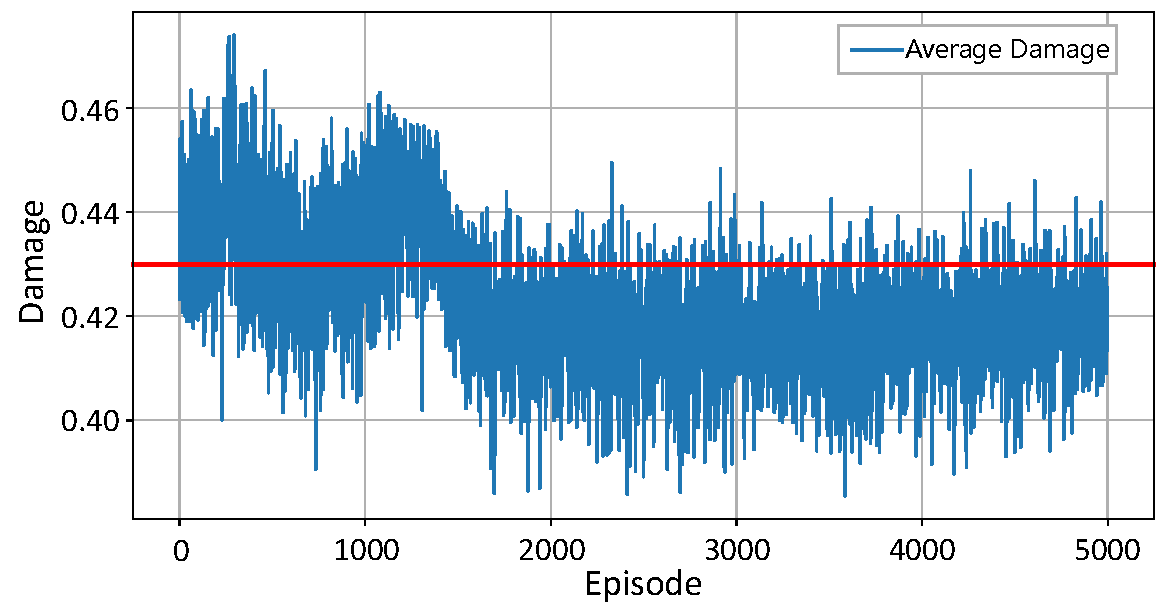
\includegraphics[width=\linewidth]{damage-1.pdf}
        \caption{Damage}
        \label{fig:damage_b}
    \end{subfigure}
    \caption{Training parameter over epochs.}
    \label{fig:combined_curves}
\end{figure}


% \begin{figure}[htbp]
% \centerline{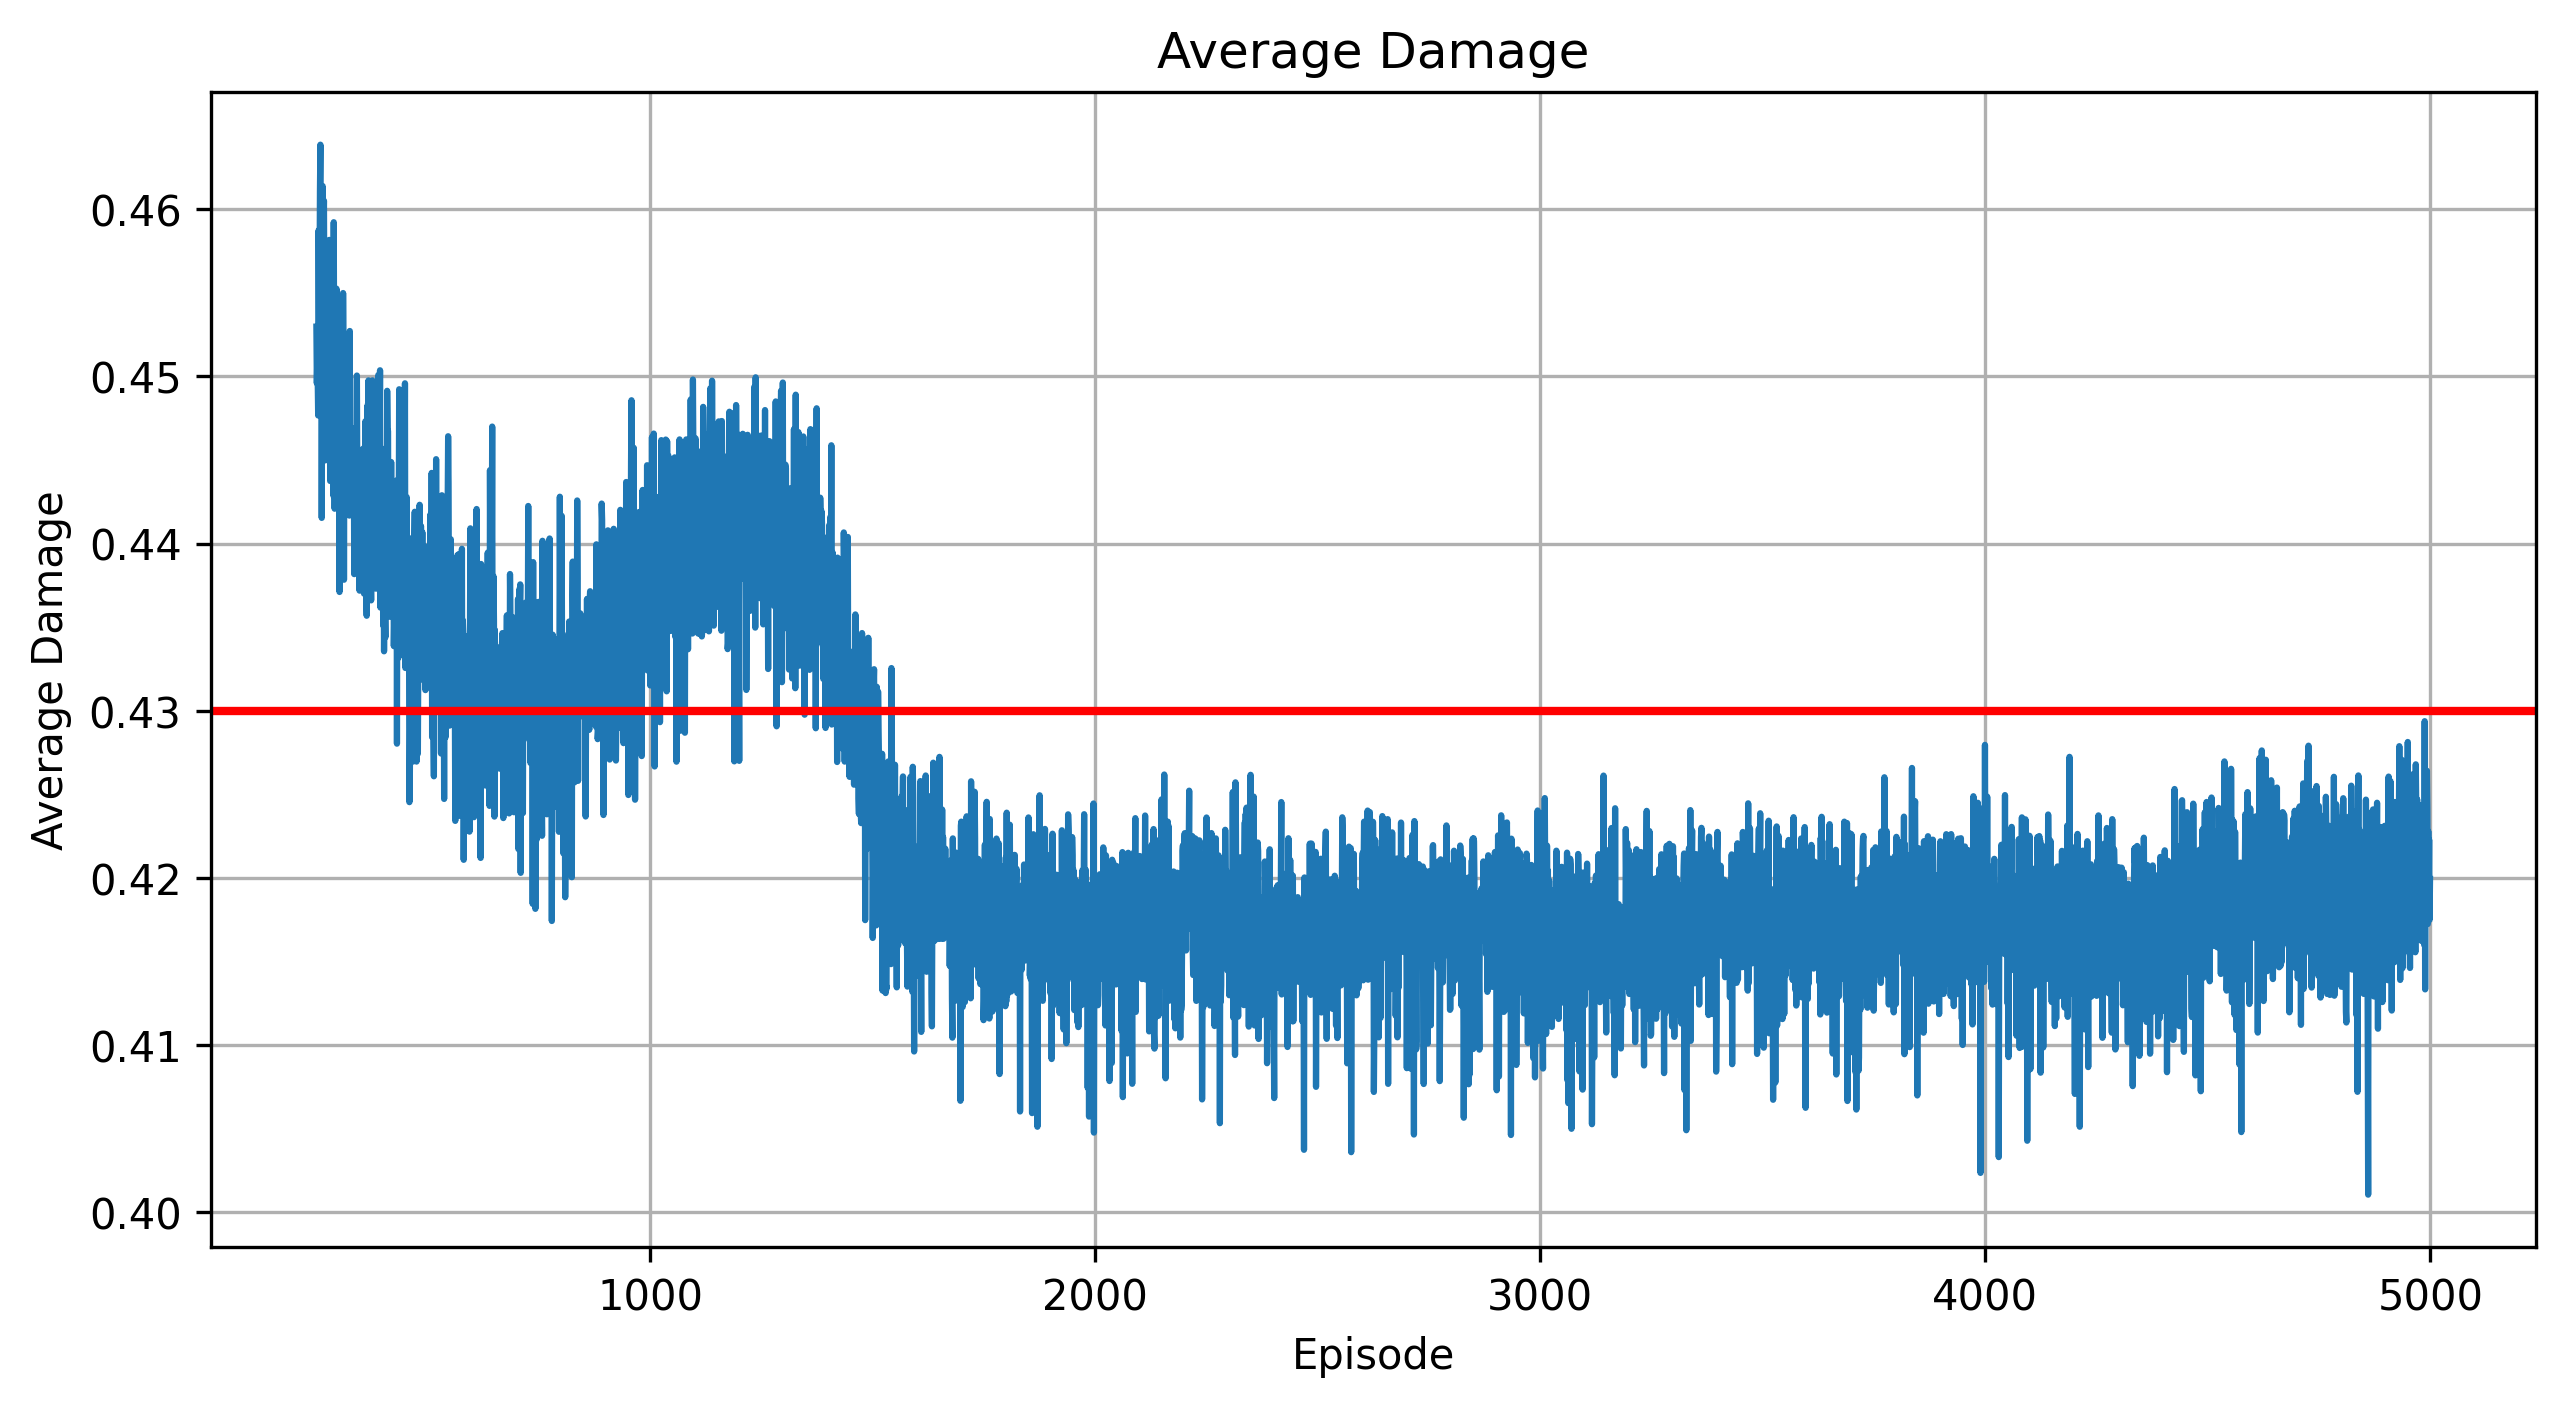
\includegraphics[width=\linewidth]{damages_episode_4999.png}}
% \caption{Example of a figure caption.}
% \label{fig:damages_episode_4999}
% \end{figure}

% 图\ref{fig:NetworkSpeed_a}展示了不同温度场下的速度曲线。当温度从$474^{\circ}C$升至$500^{\circ}C$时，速度曲线加速段提前，锻造时间缩短，表明决策网络能根据温度自适应调整策略，以应对材料高温软化特性。

Fig. \ref{fig:NetworkSpeed_a} presents the speed profiles under
different temperature fields. As the temperature increases from
$474\,^{\circ}\mathrm{C}$ to $500\,^{\circ}\mathrm{C}$, the acceleration
phase of the speed curve occurs earlier, reducing the total forging
time. This demonstrates the policy network's ability to adaptively
adjust the strategy based on temperature, effectively responding to the
material's high-temperature softening characteristics.

% \begin{figure}[htbp]
% \centerline{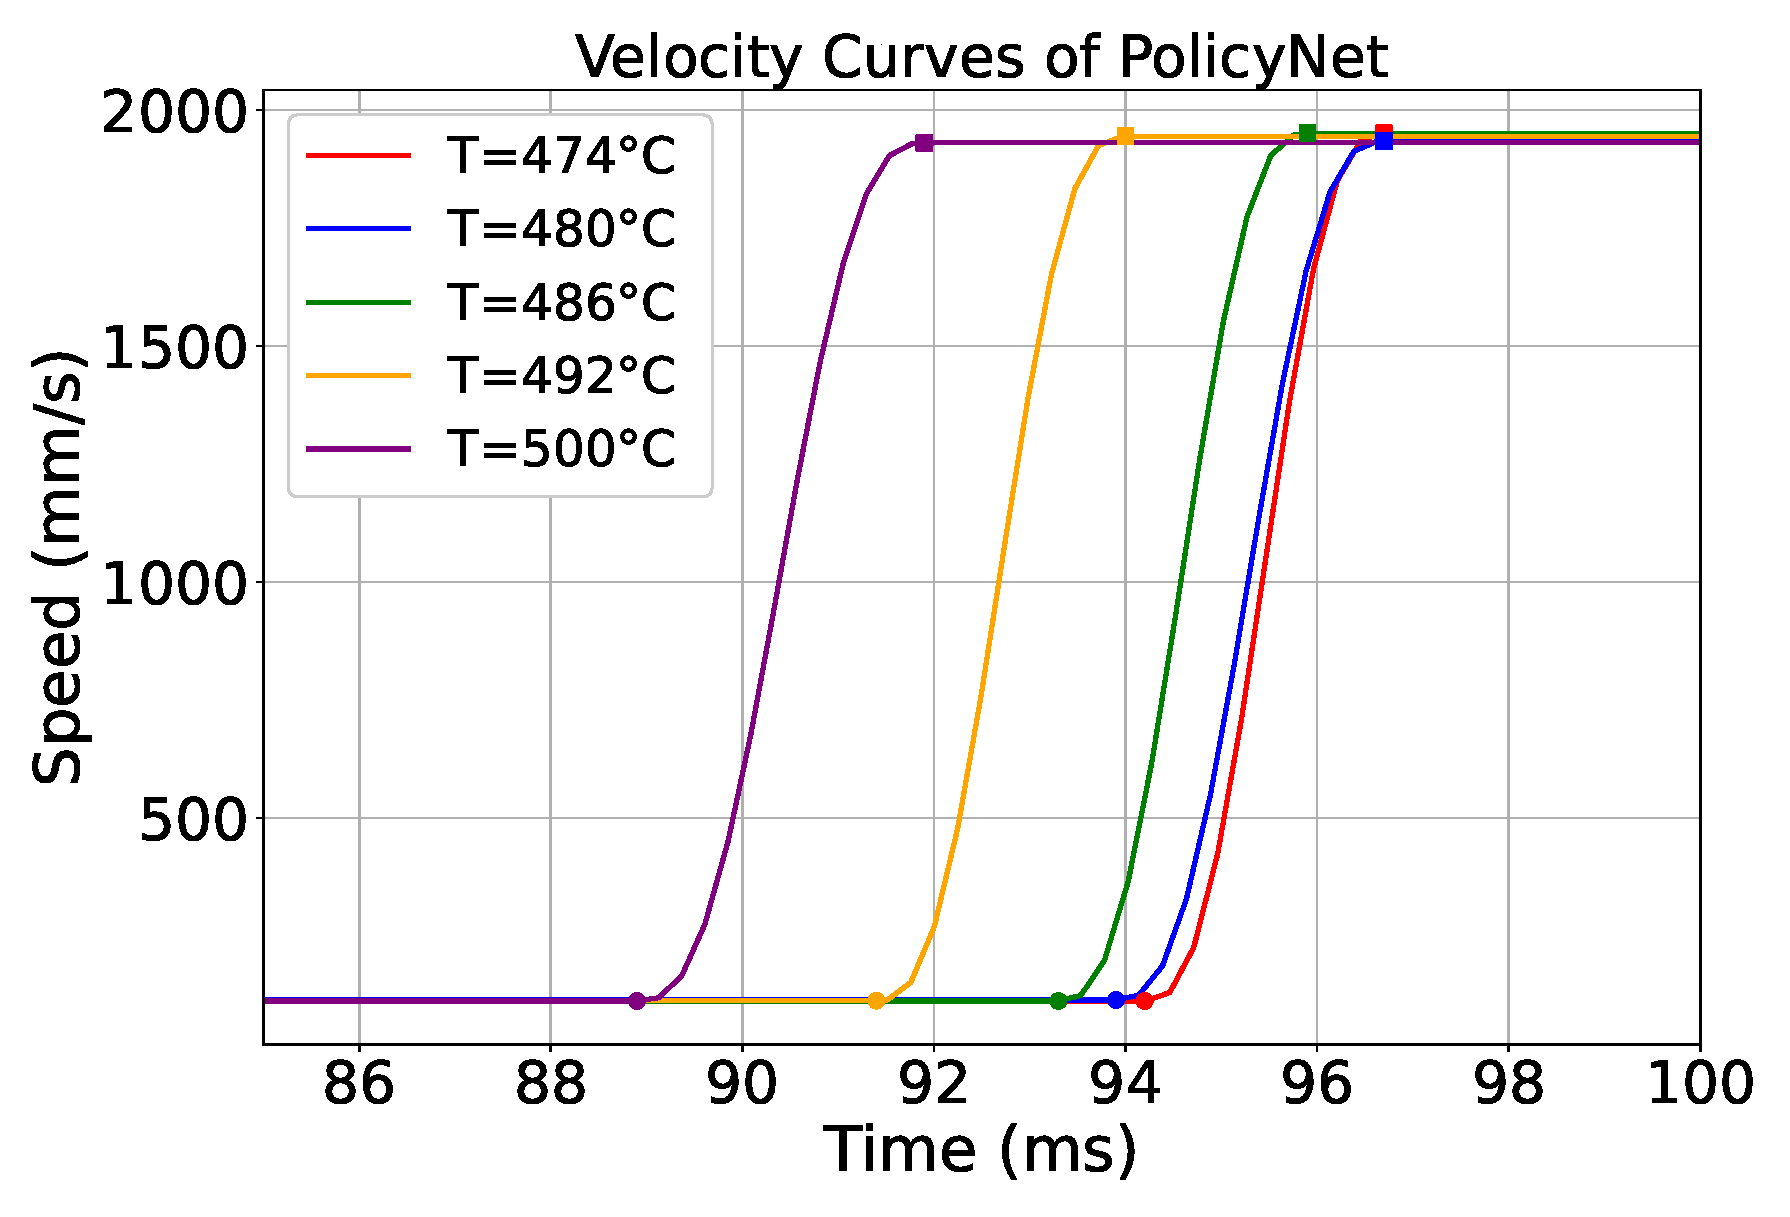
\includegraphics[width=\linewidth]{NetworkSpeed.eps}}
% \caption{Action Curves of the Policy Network Generated at  Different Temperatures (474°C, 480°C, 486°C, 492°C, 500°C).}
% \label{fig:NetworkSpeed}
% \end{figure}

% 与粒子群优化（PSO）算法\cite{wang2018particle}的对比揭示了二者特性的差异。如图\ref{fig:PSOSpeed_b}所示，PSO倾向于生成加速更早的速度曲线，导致锻造时间更短。

A comparison with the particle swarm optimization (PSO) algorithm
\cite{wang2018particle} reveals distinct characteristics between the two
approaches. As shown in Fig. \ref{fig:PSOSpeed_b}, PSO tends to generate
speed profiles with earlier acceleration phases, resulting in shorter
forging times.

% \begin{figure}[htbp]
% \centerline{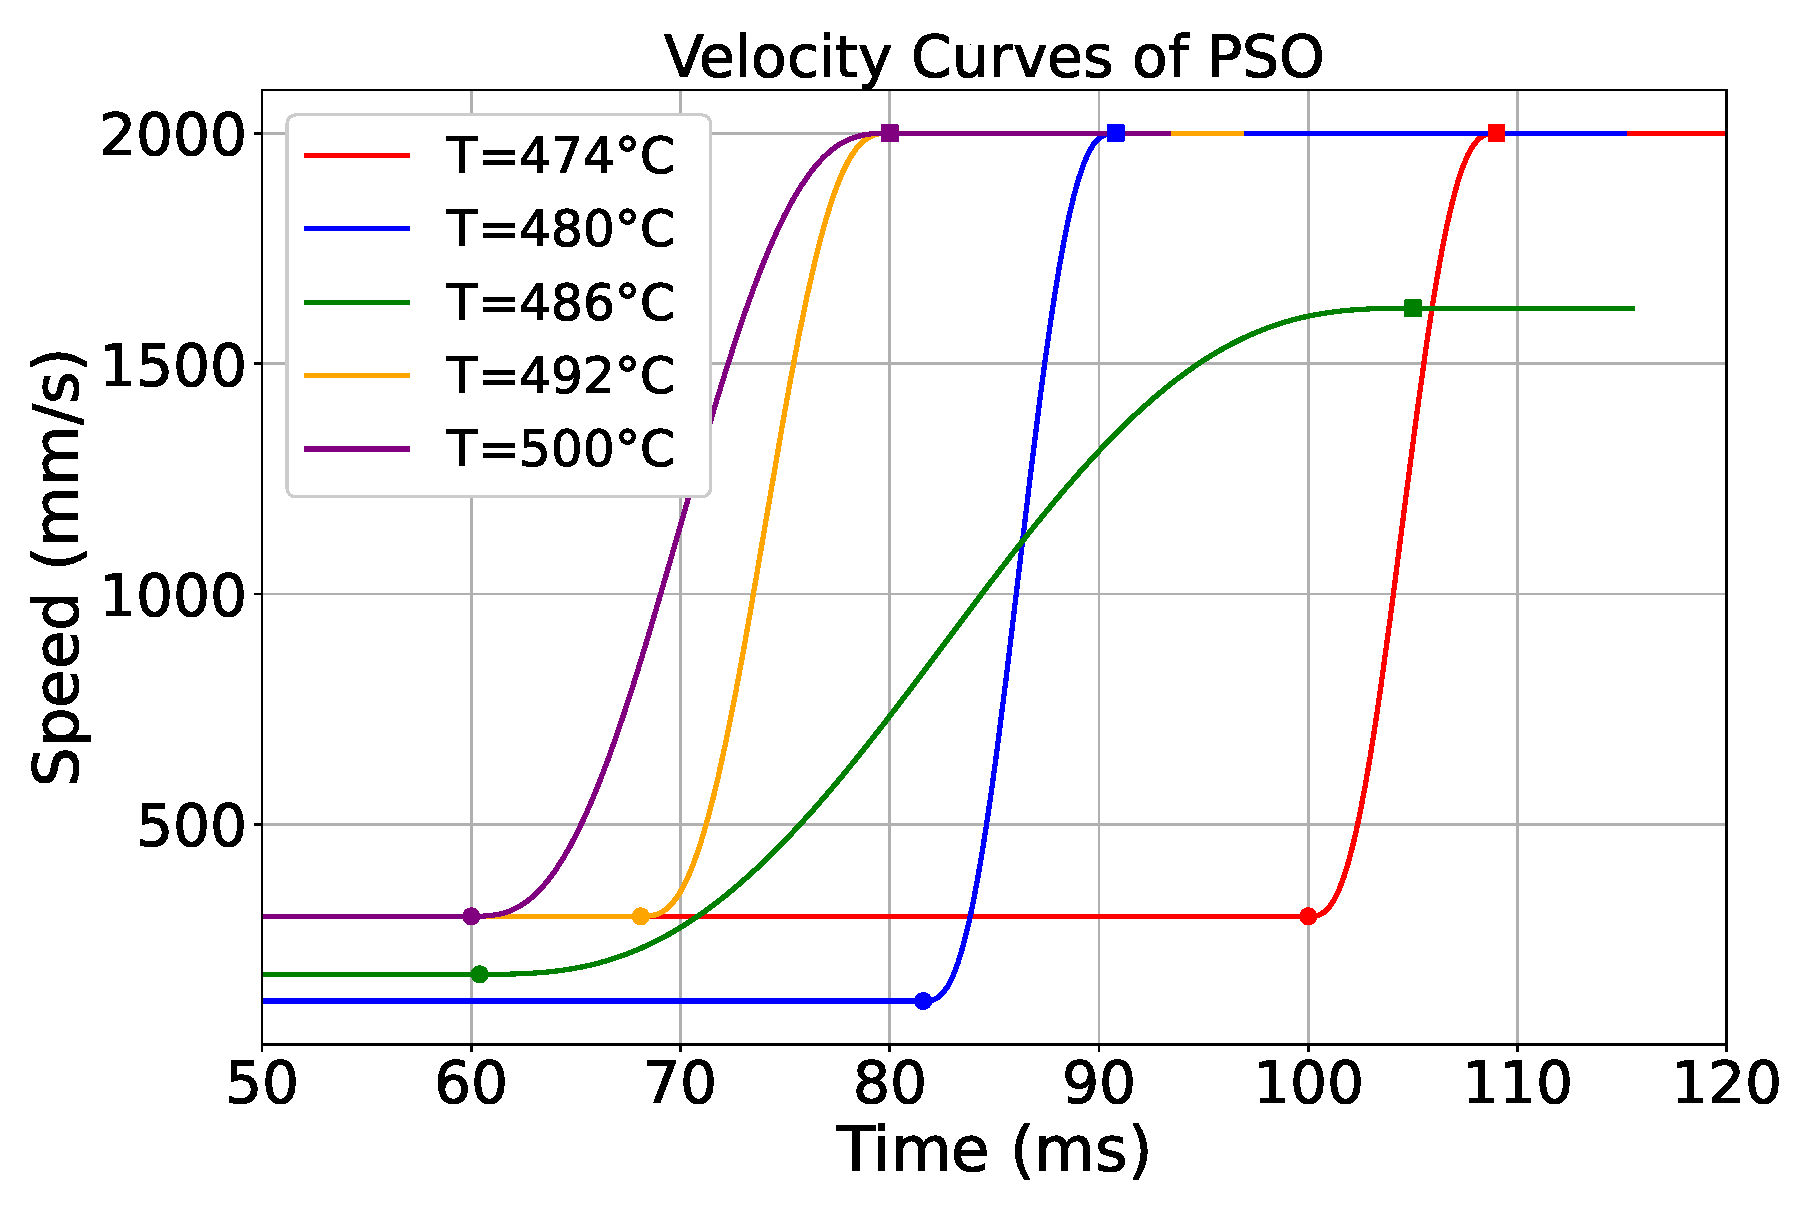
\includegraphics[width=\linewidth]{PSOSpeed.eps}}
% \caption{Action Curves of the PSO Generated at  Different Temperatures (474°C, 480°C, 486°C, 492°C, 500°C).}
% \label{fig:PSOSpeed}
% \end{figure}



% \begin{figure}[htbp]
%     \centering
%     \begin{minipage}{0.48\columnwidth}
%         \centering
%         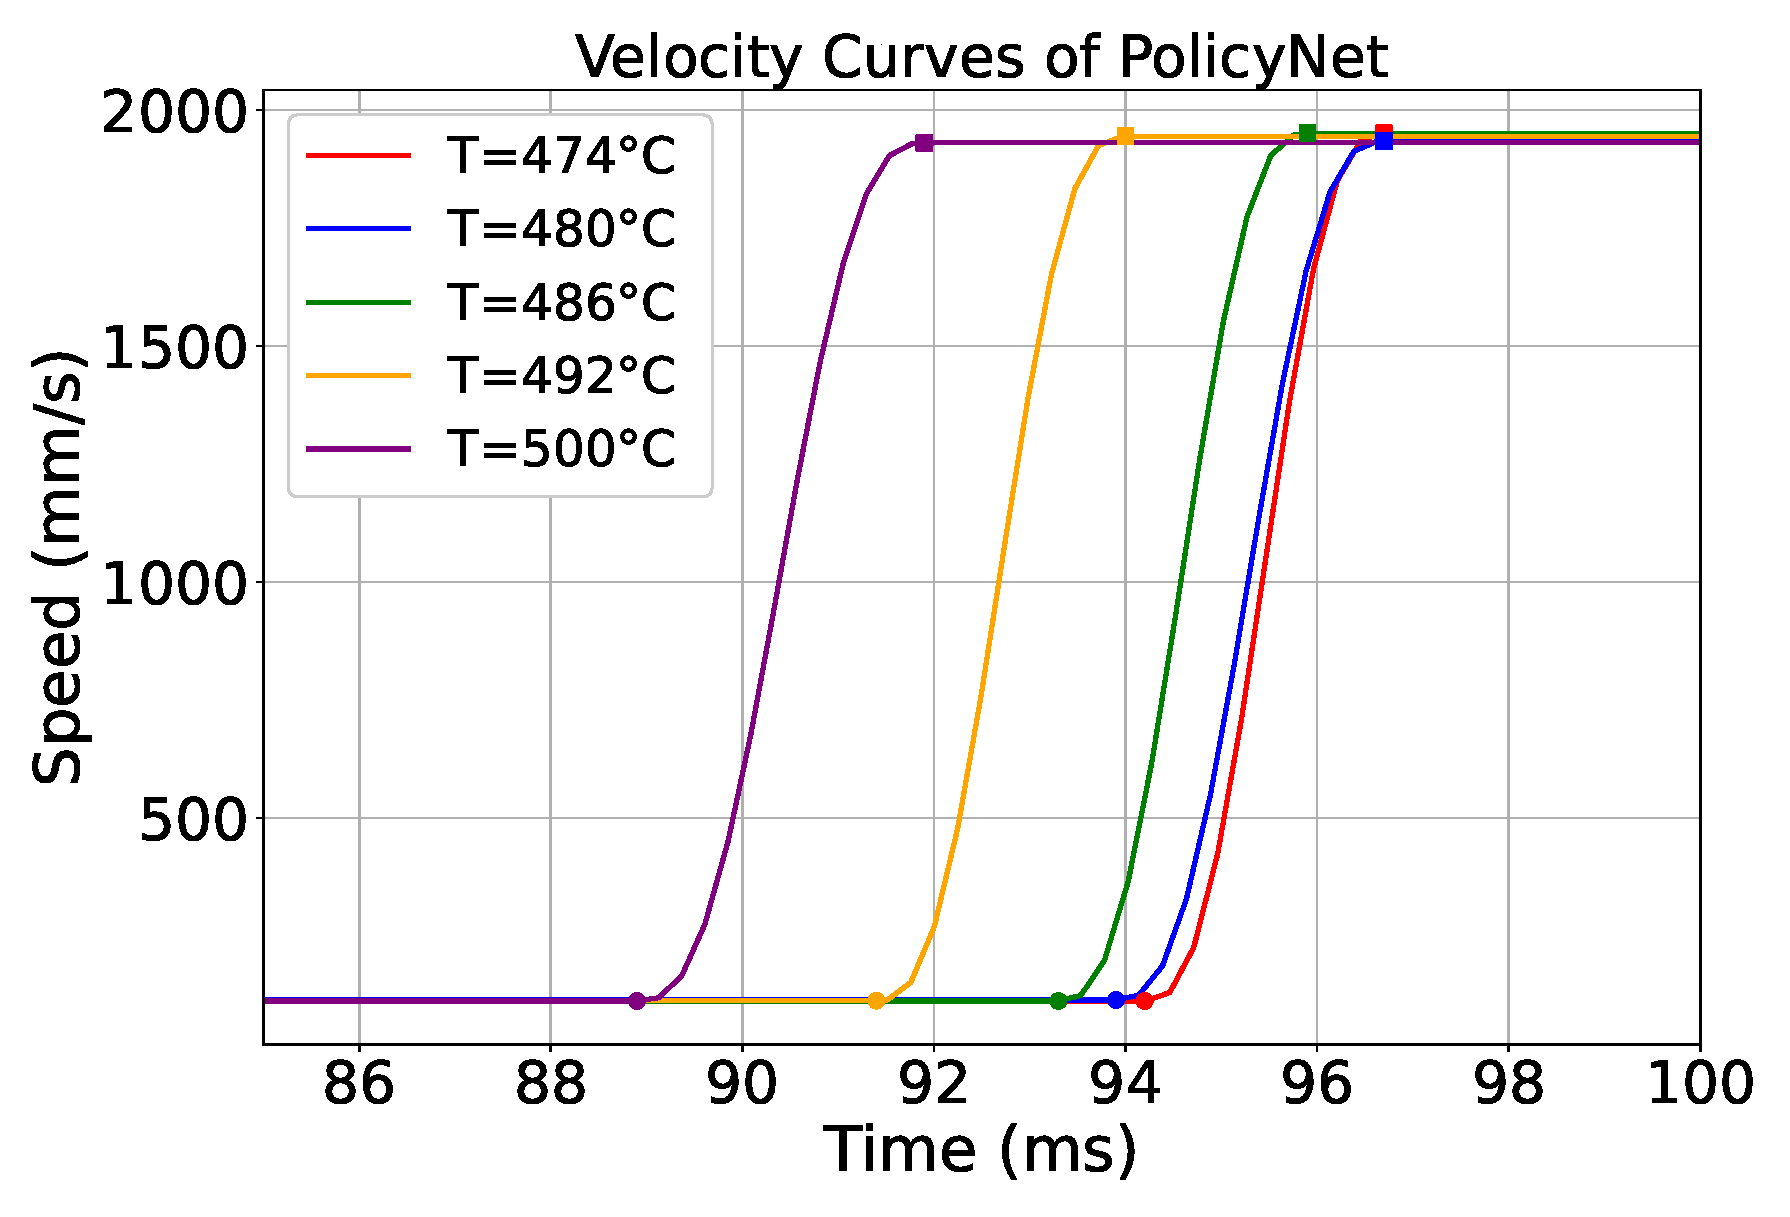
\includegraphics[width=\linewidth]{NetworkSpeed.eps}
%         \caption{Action Curves of the Policy Network Generated at Different Temperatures (474°C, 480°C, 486°C, 492°C, 500°C).}
%         \label{fig:NetworkSpeed}
%     \end{minipage}
%     \hfill
%     \begin{minipage}{0.48\columnwidth}
%         \centering
%         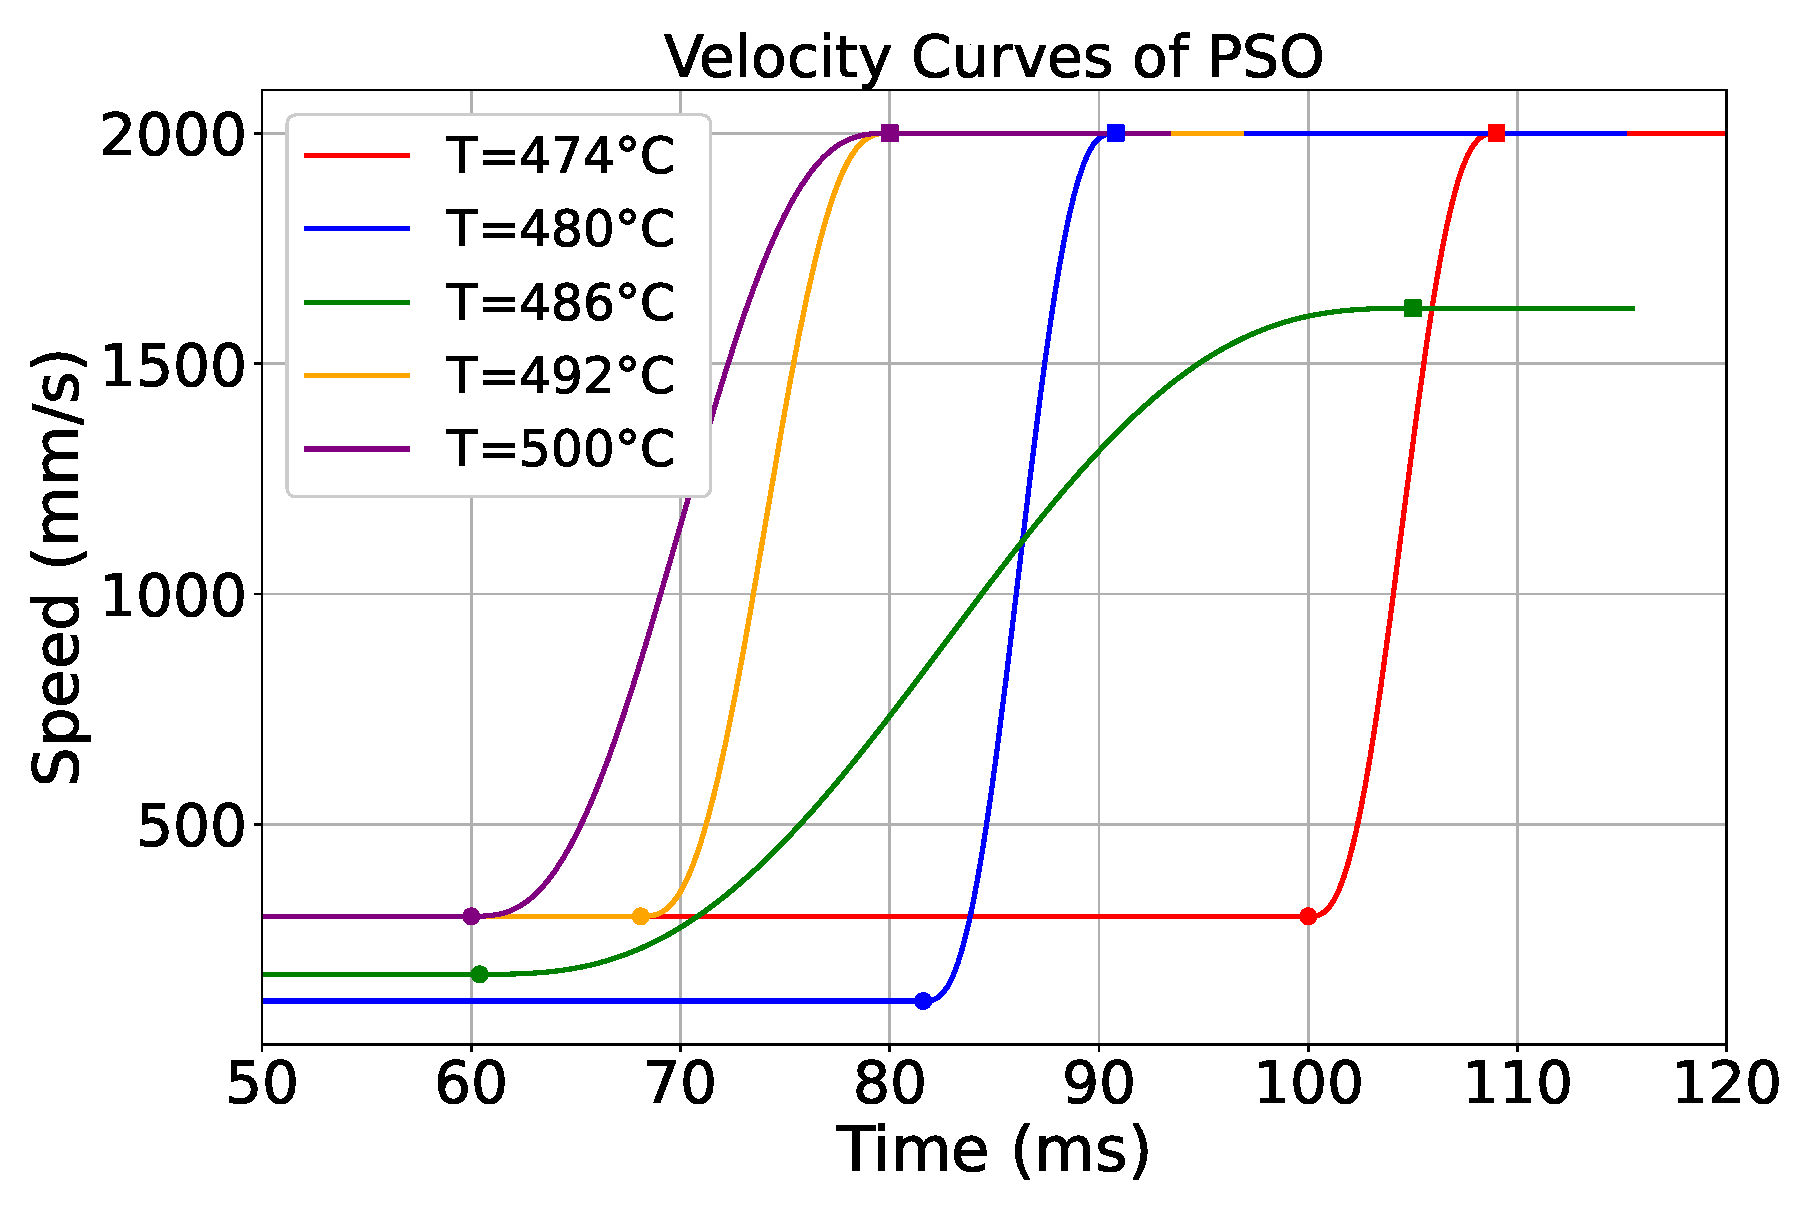
\includegraphics[width=\linewidth]{PSOSpeed.eps}
%         \caption{Action Curves of the PSO Generated at Different Temperatures (474°C, 480°C, 486°C, 492°C, 500°C).}
%         \label{fig:PSOSpeed}
%     \end{minipage}
% \end{figure}


\begin{figure}[htbp]
    \centering
    \begin{subfigure}{0.48\columnwidth}
        \centering
        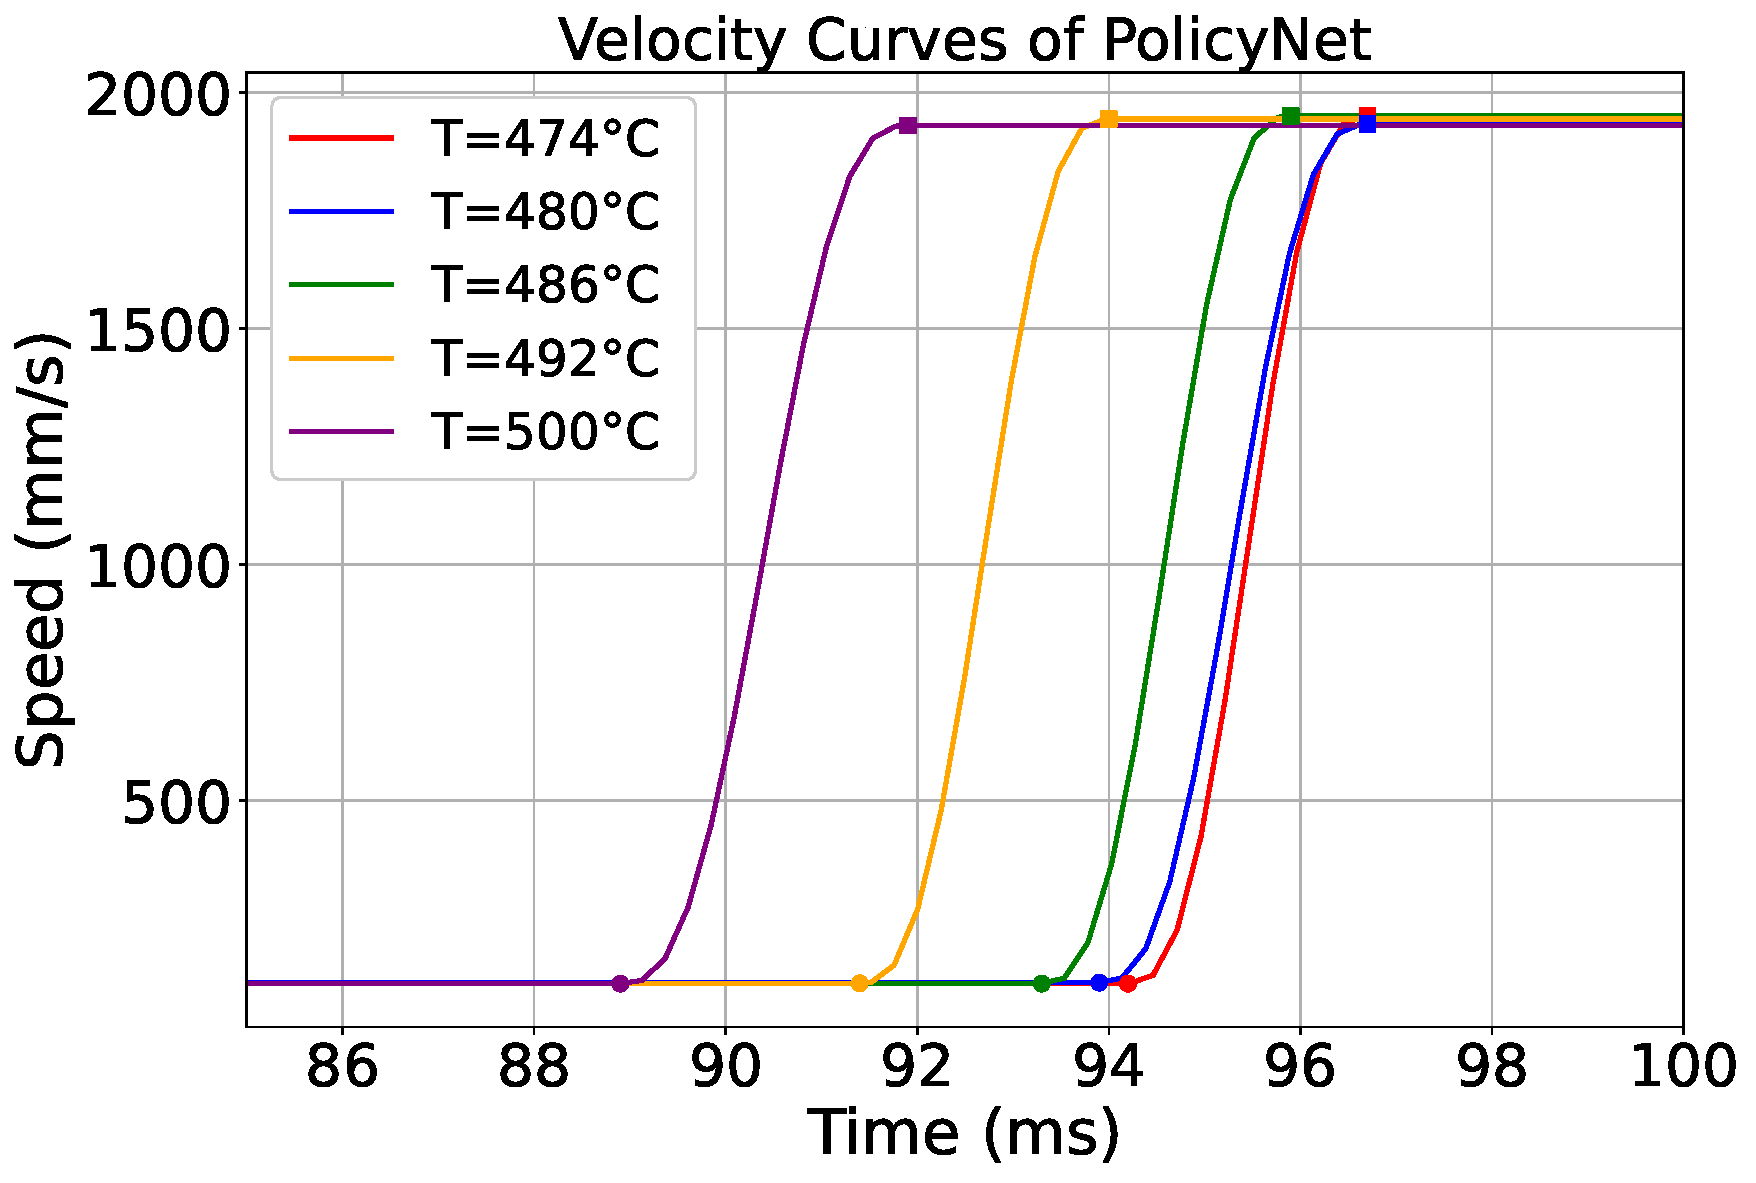
\includegraphics[width=\linewidth]{NetworkSpeed.pdf}
        \caption{Policy Network}
        \label{fig:NetworkSpeed_a}
    \end{subfigure}
    \hfill
    \begin{subfigure}{0.48\columnwidth}
        \centering
        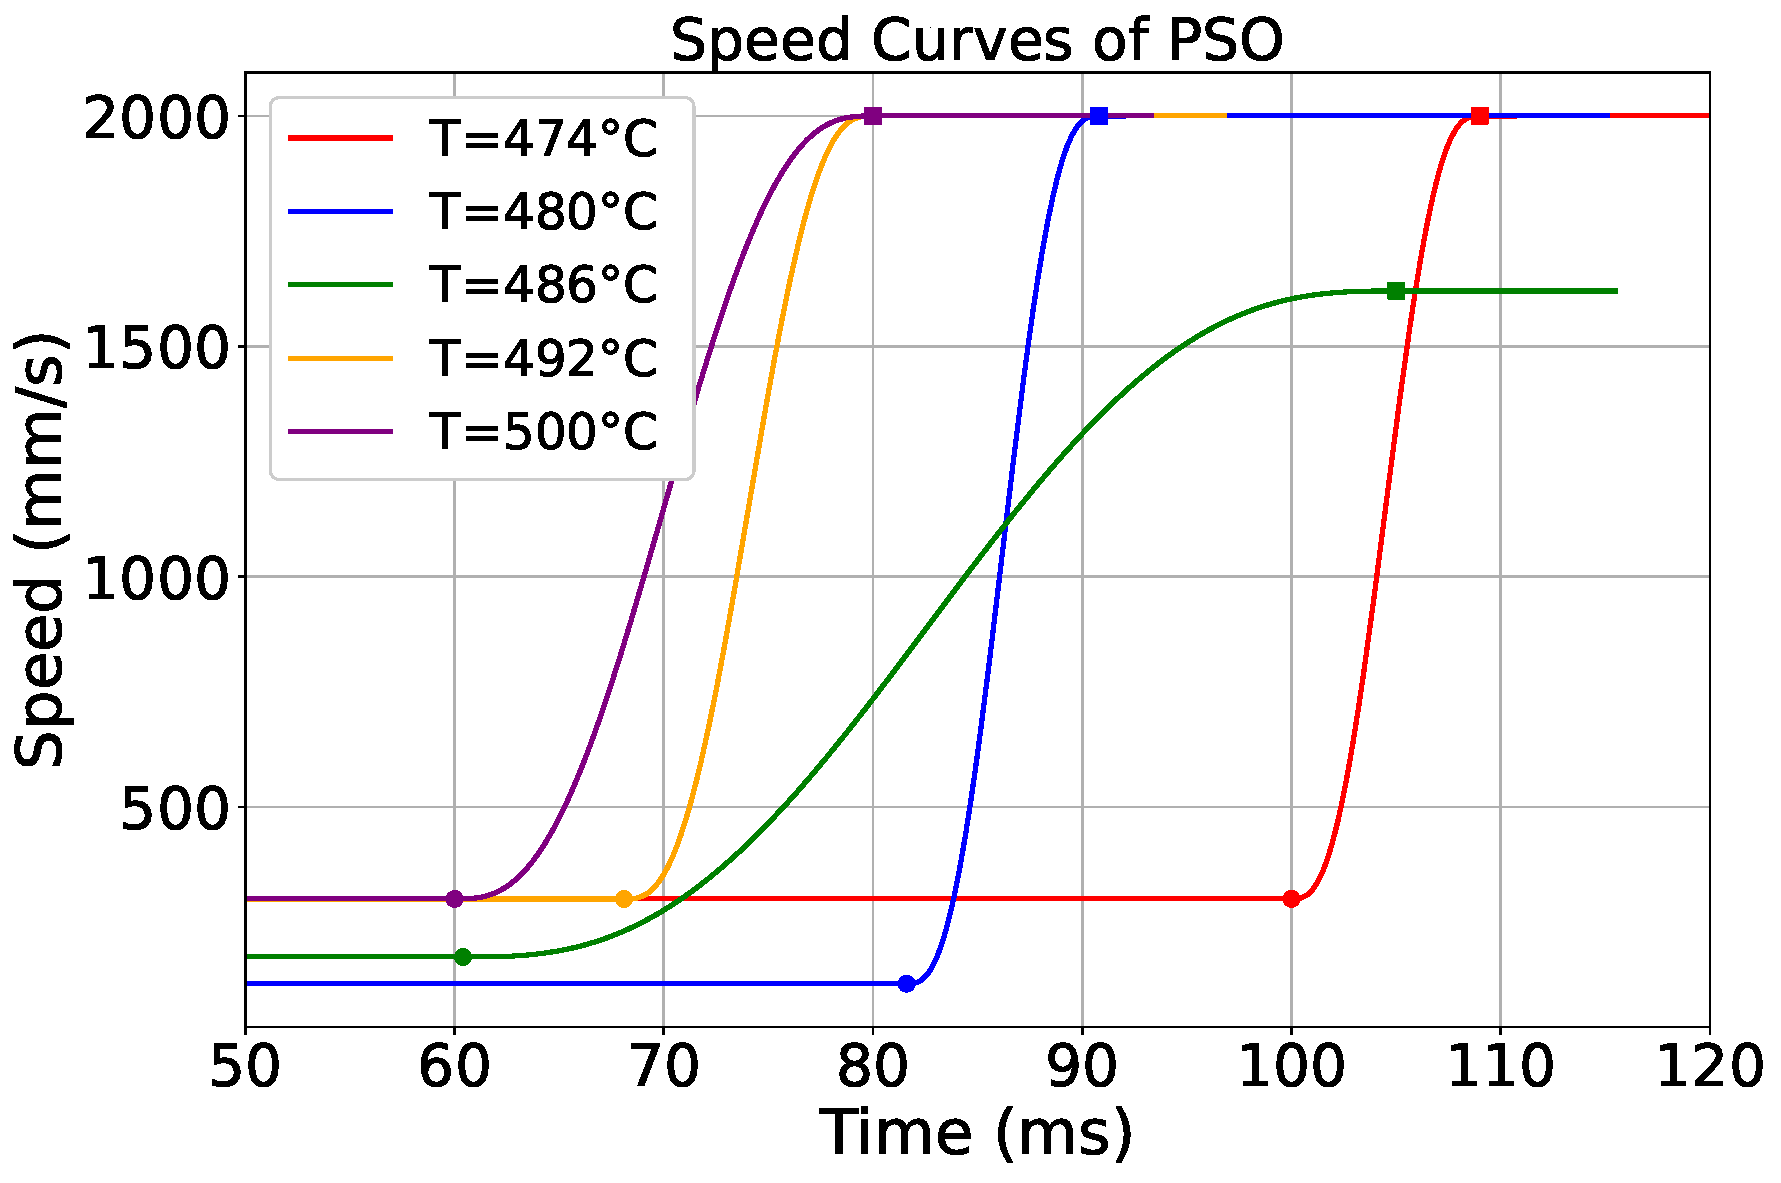
\includegraphics[width=\linewidth]{PSOSpeed.pdf}
        \caption{PSO}
        \label{fig:PSOSpeed_b}
    \end{subfigure}
    \caption{Action curves generated at different temperatures (474°C, 480°C, 486°C, 492°C, 500°C). (a) Policy network; (b) Particle swarm optimization.}
    \label{fig:combined_curves}
\end{figure}

% 工艺性能上（表\ref{tab:Method Comparison}），PSO在锻造时间与损伤率（$0\%$，决策网络为$8\%$）上略优。决策效率上，PSO需约$0.9\text{s}$达到决策网络性能（图\ref{fig:PSO-Objective}），$2.5\text{s}$达最优，而决策网络仅需$0.097\text{s}$，效率相差近一个数量级。

In terms of process performance (Table \ref{tab:Method Comparison}), PSO
slightly outperforms in forging time and achieves a lower damage rate
($0\%$ vs. $8\%$ for the policy network). Regarding decision efficiency,
PSO requires approximately $0.9\text{s}$ to reach the performance level
of the policy network (Fig. \ref{fig:PSO-Objective}) and $2.5\text{s}$ to
achieve its optimum, whereas the policy network requires only
$0.097\text{s}$—nearly an order of magnitude faster.

\begin{table}[htbp]
\centering
\caption{Method Comparison}
\setlength{\tabcolsep}{3.5pt} % 缩小列间距（默认约6pt，可根据需要调整）
\begin{tabular}{c c c c}
\toprule
\textbf{Method} & \textbf{Forge Time} & \textbf{Decision Time} & \textbf{Damage Rate}\\
& (mean$\pm$std,ms) & (mean$\pm$std,ms) & (\%)\\
\midrule
PolicyNet & 121.91 $\pm$ 6.63 & 97.37 $\pm$ 3.86 & 8.00 \\
PSO       & 108.72 $\pm$ 11.55 & 2580 $\pm$ 1370  & 0.00 \\
\bottomrule
\end{tabular}
\label{tab:Method Comparison}
\end{table}


\begin{figure}[htbp]
\centerline{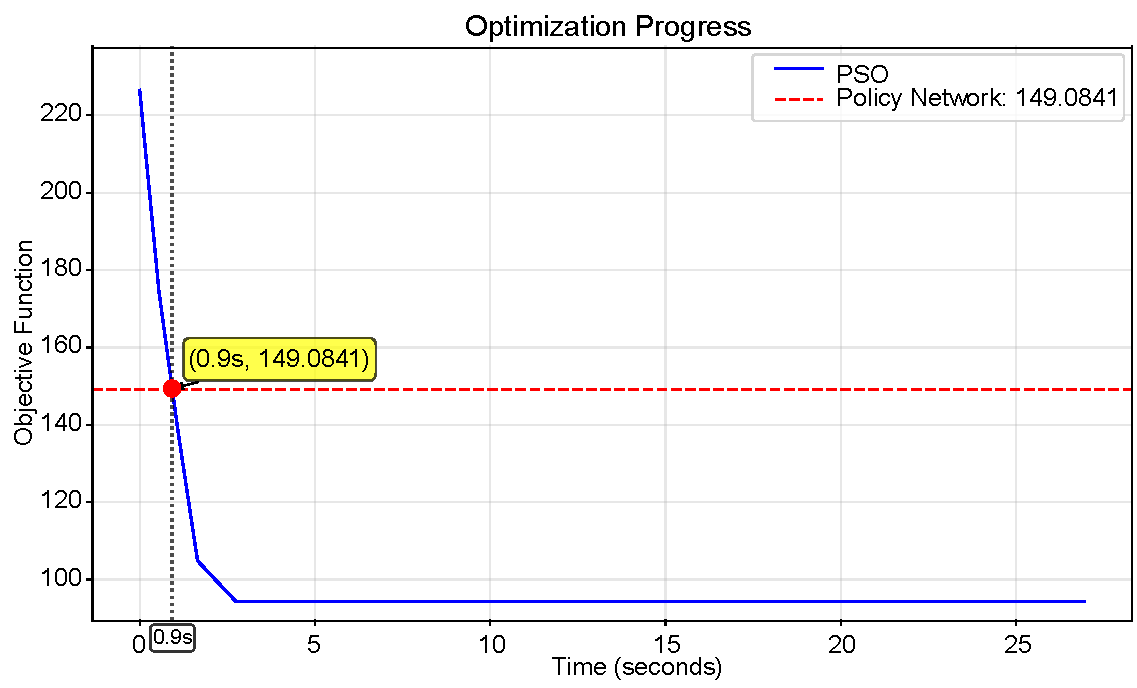
\includegraphics[width=\linewidth]{PSO-Objective-2.pdf}}
\caption{Objective function comparison.}
\label{fig:PSO-Objective}
\end{figure}
In summary, while PSO achieves superior process quality, its extended
decision time hinders real-time application. In contrast, the policy
network provides rapid decision-making while maintaining acceptable
process quality, demonstrating greater suitability for practical
scenarios.
